%Para slide em "Wide-Screen" usar:
\documentclass[aspectratio=43,10pt]{beamer} 

%Para slide "quadrado" usar:
%\documentclass{beamer} 

\usepackage{tikz}

%Elaborado por Mateus Moro Lumertz

\author{mateuslumertz}
\definecolor{cor1}{RGB}{0,100,166}
\definecolor{cor2}{RGB}{100,195,213}
\definecolor{cor5}{RGB}{150,203,226}
\definecolor{cor3}{RGB}{30,130,186}
\definecolor{cor4}{RGB}{40,185,218}
\definecolor{preto}{RGB}{0,0,0}
\definecolor{branco}{RGB}{255,255,255}
% Configuração das Cores
\setbeamercolor{paleta1}{fg=cor1,bg=white}
\setbeamercolor{paleta2}{fg=cor1,bg=white}
\setbeamercolor{estrutura}{fg=cor1,bg=white}
\setbeamercolor{titulo_rodape}{fg=black,bg=white}
\setbeamercolor{data_rodape}{fg=gray,bg=white}
\setbeamercolor{frametitle}{fg=branco,bg=cor1}

% Modelo do rodapé
\defbeamertemplate*{footline}{mytheme}{%
  \leavevmode%
  \hbox{\begin{beamercolorbox}[wd=.5\paperwidth,ht=2.5ex,dp=1.125ex,leftskip=.3cm,rightskip=.3cm]{titulo_rodape}%
    \makebox[2em][l]{{\usebeamerfont{titulo_rodape}\textcolor{cor1}{\insertframenumber}}}%
    {\usebeamercolor{titulo_rodape}\insertshorttitle}
  \end{beamercolorbox}%
  \begin{beamercolorbox}[wd=.2\paperwidth,ht=2.5ex,dp=1.125ex,leftskip=.3cm,rightskip=.3cm]{data_rodape}%
    \usebeamerfont{data_rodape}\insertshortdate%
  \end{beamercolorbox}%
  \begin{beamercolorbox}[wd=.3\paperwidth,ht=2.5ex,dp=1.125ex,leftskip=.3cm,rightskip=.3cm,right]{titulo_rodape}%
    
\includegraphics[width=.2\paperwidth,height=7ex,keepaspectratio]{imagens/logo.png}\hspace*{2em}%
  \end{beamercolorbox}}%
  \vskip0pt%
}

% Slide de Título
\defbeamertemplate*{title page}{mytheme}[1][]
{%
  \begin{tikzpicture}[remember picture,overlay]
    \filldraw[cor1]
    (current page.north west) --
    ([yshift=-12cm]current page.north west) --
    ([xshift=-4cm,yshift=-12cm]current page.north east) {[rounded corners=15pt]--
    ([xshift=-4cm,yshift=3cm]current page.south east)} --
    ([yshift=3cm]current page.south west) --
    (current page.south west) --
    (current page.south east) --
    (current page.north east) -- cycle
    ;
  \filldraw[branco]
    (current page.north west) --
    ([yshift=-2.15cm]current page.north west) --
    ([xshift=-3cm,yshift=-2.15cm]current page.north east) {[rounded corners=15pt]--
    ([xshift=-3cm,yshift=3cm]current page.south east)} --
    ([yshift=3cm]current page.south west) --
    (current page.south west) --
    (current page.south east) --
    (current page.north east) -- cycle
    ;
    \filldraw[cor2]
    ([xshift=-0.25cm,yshift=3cm]current page.south east)--
    ([xshift=-2.75cm,yshift=3cm]current page.south east)--
    ([xshift=-2.75cm,yshift=3.85cm]current page.south east)--
    ([xshift=-0.25cm,yshift=3.85cm]current page.south east)-- cycle
    ;
    \filldraw[cor3]
    ([xshift=-0.25cm,yshift=4cm]current page.south east)--
    ([xshift=-2.75cm,yshift=4cm]current page.south east)--
    ([xshift=-2.75cm,yshift=4.85cm]current page.south east)--
    ([xshift=-0.25cm,yshift=4.85cm]current page.south east)-- cycle
    ;
    \filldraw[cor4]
    ([xshift=-0.25cm,yshift=5cm]current page.south east)--
    ([xshift=-2.75cm,yshift=5cm]current page.south east)--
    ([xshift=-2.75cm,yshift=5.85cm]current page.south east)--
    ([xshift=-0.25cm,yshift=5.85cm]current page.south east)-- cycle
    ;
    \filldraw[cor5]
    ([xshift=-0.25cm,yshift=6cm]current page.south east)--
    ([xshift=-2.75cm,yshift=6cm]current page.south east)--
    ([xshift=-2.75cm,yshift=6.85cm]current page.south east)--
    ([xshift=-0.25cm,yshift=6.85cm]current page.south east)-- cycle
    ;
  \node[text=branco,anchor=south west,font=\sffamily\LARGE,text width=.68\paperwidth] 
  at ([xshift=10pt,yshift=-0.5cm]current page.west)
  (title)
  {\raggedright\inserttitle};  
  
  \node[text=cor1,anchor=south west,font=\sffamily\small,text width=.75\paperwidth] 
  at ([xshift=10pt,yshift=3.6cm]current page.west)
  (title)
  {\raggedright Université Côte d'Azur};  
  
  \node[anchor=east]
  at ([xshift=-0.15cm,yshift=-1cm]current page.north east)
  {
\includegraphics[width=2.5cm]{imagens/logo.png}};
  
  \node[text=preto,font=\large\sffamily,anchor=south west]
  at ([xshift=30pt,yshift=0.5cm]current page.south west)
  (date)
  {\insertdate};
  \node[text=preto,font=\large\sffamily,anchor=south west]
  at ([yshift=5pt]date.north west)
  (author)
  {\insertauthor};
  \end{tikzpicture}%
}

% remove navigation symbols
\setbeamertemplate{navigation symbols}{}

% definition of the itemize templates
\setbeamertemplate{itemize item}[circle]
\setbeamercolor{itemize item}{fg=cor3,bg=white}
\setbeamercolor{itemize subitem}{fg=cor4,bg=white}
\setbeamercolor{itemize subsubitem}{fg=cor2,bg=white}

%%%%%%%%%%%%%%%%%%%%%%%%%%%%%%%%%%%%%%%%%%%%%%%%%%%%%%%%%%%%%%%%%%%%
%%%%%%%%%%%%%%%%%%%%%%%%%%%%%%%%%%%%%%%%%%%%%%%%%%%%%%%%%%%%%%%%%%%%
%%%%%%%%%%%%%%%%%%%%%%%%%%%%%%%%%%%%%%%%%%%%%%%%%%%%%%%%%%%%%%%%%%%%
%%%%%%%%%%%%%%%%%%%%%%%%%%%%%%%%%%%%%%%%%%%%%%%%%%%%%%%%%%%%%%%%%%%%
%%%%%%%%%%%%%%%%%%%%%%%%%%%%%%%%%%%%%%%%%%%%%%%%%%%%%%%%%%%%%%%%%%%%

\title[Choropleth map on WASABI]{Choropleth map exploration of the WASABI music dataset}
\author{Quentin Le Roux}
\date{\today}

\begin{document}

\begin{frame}[plain]
\maketitle
\end{frame}

%Slide 
\begin{frame}
    \frametitle{Introduction}
    \framesubtitle{Why a choropleth map for music data}
    
    \begin{itemize}
        \item A Choropleth map displays geographical areas that are coloured in relation to a variable. It allows to highlight patterns across the displayed location.
        \item Very common to see in news media, such as in music
        \item Example in The Atlantic:
        \begin{center}
            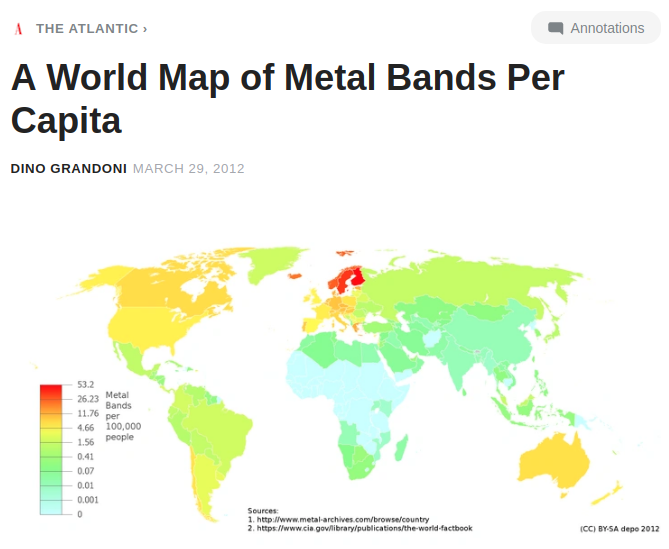
\includegraphics[width=0.6\linewidth]{imagens/atlantic_article.png}
        \end{center}
    \end{itemize}
\end{frame}

%Slide 
\begin{frame}
    \frametitle{Implementation}
    \framesubtitle{Presentation of the choropleth map implementation}
    \begin{itemize}
        \item \textbf{Goal}: reproduce \& expand the visualization found in news media
        \item We want to show the countries with the most country bands per capita, \textbf{per genres and decades since the 1960s}.
    \end{itemize}
    \newline
    \newline
    \begin{center}
       \textit{Let's launch the visualization!}
    \end{center}
    \newline
    \newline
    \textbf{On a terminal}:
    \newline
    \newline
    \small{
    \$ git clone https://github.com/LMquentinLR/choropleth\_wasabi\_dataset.git
    
    
    \$ sudo apt install npm
    
    
    \$ npm i
    
    
    \$ sudo npm install -g parcel-bundler
    
    
    \$ parcel index.html}
\end{frame}

%Slide 
\begin{frame}
    \frametitle{Possible interactions with the map}
    \framesubtitle{What can it do?}
    Tooltips per countries! Interactivity! Animation!
    \newline\newline
    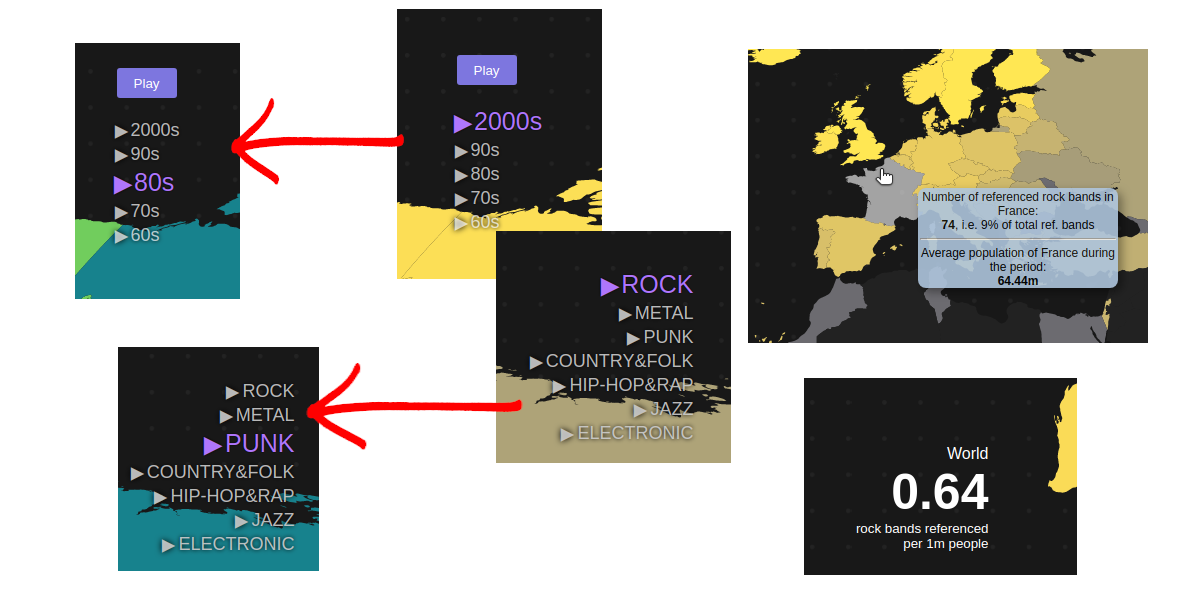
\includegraphics[width=1\linewidth]{imagens/interactions.png}
\end{frame}

%Slide 
\begin{frame}
    \frametitle{How does it work?}
    \framesubtitle{Folder Structure}
    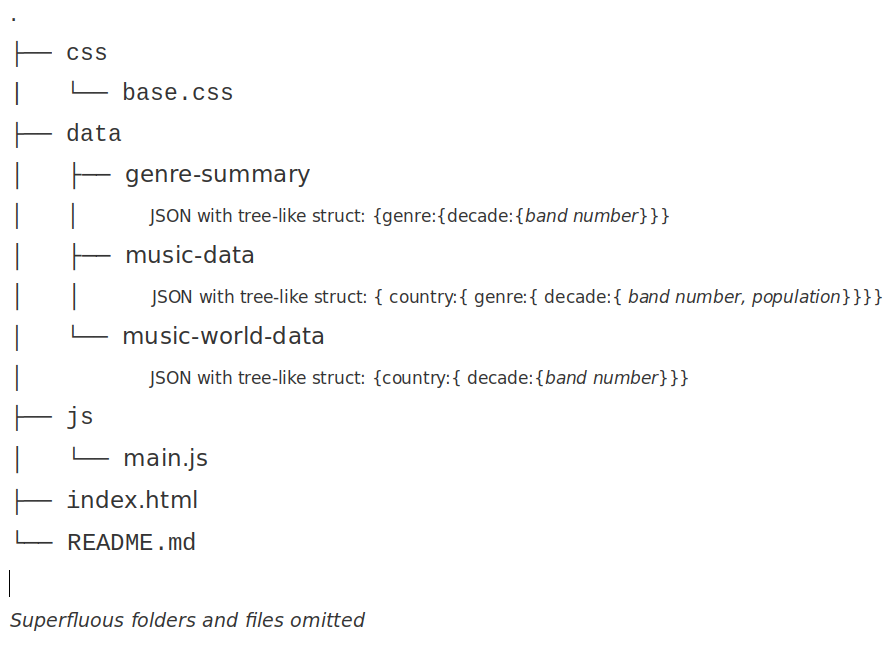
\includegraphics[width=1\linewidth]{imagens/folder_structure.png}
\end{frame}

%Slide 
\begin{frame}
    \frametitle{How does it work?}
    \framesubtitle{Data Consumption by D3.js}
    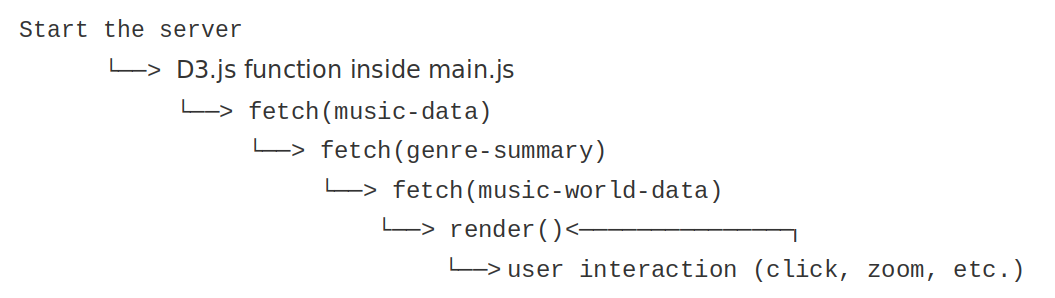
\includegraphics[width=1\linewidth]{imagens/action.png}
\end{frame}

%Slide 
\begin{frame}
    \frametitle{Data processing}
    \framesubtitle{Datasets used}
        \textbf{WASABI dataset}. Tables used:
        \begin{itemize}
            \item \textsc{Albums}, used attributes: \textsc{\_id}, \textsc{location.country}
            \item \textsc{Artists}, used attributes: \textsc{id\_artist}, \textsc{genre}, \textsc{publicationDate}
        \end{itemize}
        \textbf{World Bank population dataset}
        \begin{itemize}
            \item Used attributes: \textsc{Year}, \textsc{Country.Code}, \textsc{Country.Name}
        \end{itemize}
\end{frame}

%Slide 
\begin{frame}
    \frametitle{Data processing}
    \framesubtitle{Processing Pipeline - 1}
    \small{
        \begin{enumerate}
            \item Simplify \textsc{genres} in the \textsc{Artists} table by generalizing the values (e.g. 'punk rock', 'math rock', etc. $\rightarrow$ 'rock')
            \item Remove rows not sorted into genre families: "rock", "metal", "punk", "country/folk", "hiphop/rap", "jazz", "electro"
            \item Lower-case all string data
            \item Transform all \textsc{publicationDate} (i.e. years) into \textsc{decades} (e.g. $\{1980, ..., 1989\} \rightarrow 1980$)
            \item \textsc{Albums} and \textsc{Artists} tables are joined via the keys \textsc{\_id} and \textsc{id\_artist}
            \item \textsc{location.country} and \textsc{country.name} are standardized and used as keys to join the \textsc{wasabi} with the \textsc{world bank} tables
            \item The resulting table is grouped by \textsc{countries}, \textsc{decades}, and \textsc{genres}
        \end{enumerate}
    }
\end{frame}

%Slide 
\begin{frame}
    \frametitle{Data processing}
    \framesubtitle{Processing Pipeline - 2}
    \small{
        We dump the data in three different JSON files with the following tree-like structure:
        \begin{itemize}
            \item genre-summary:\linebreak
            \scriptsize{\{\textsc{genre}:\{\textsc{decade}:\{\textsc{\# bands}\}\}\}}
            \item music-data:\linebreak
            \scriptsize{\{\textsc{country}:\{\textsc{genre}:\{\textsc{decade}:\{\textsc{pop.},\textsc{\# bands}\}\}\}\}}
            \item music-world-data:\linebreak
            \scriptsize{\{\textsc{country}:\{\textsc{decade}:\{\textsc{\# bands}\}\}\}}
        \end{itemize}
    The goal of such file structures is to minimize the number of computations performed by the D3.js rendering function, which renders the choropleth map. The cost is the inclusion of 2 additional JSON weighting a total of 20Kb. 
    }
\end{frame}

%Slide 
\begin{frame}
    \frametitle{Evaluation process}
    \framesubtitle{Why evaluate?}
    To summarize, a user can use the Choropleth map to perform the following:
    \begin{itemize}
        \item Explore band concentration per country, genre, and decade
        \item Access a tooltip by hovering on a country that provides demographic and market share data on a specific genre and decade
        \item Play a scrolling animation over the decade range (from the 1960s to the 2000s) for each genre
    \end{itemize}
    This can represent a \textbf{complex number of interactions}. As such, we can be \textbf{interested in evaluating how people would react to them}.
\end{frame}

%Slide 
\begin{frame}
    \frametitle{Evaluation process}
    \framesubtitle{Result example}
    \begin{itemize}
        \item 3 steps:
        \begin{itemize}
        \item Welcoming, briefing, and interview of the participants (with a questionnaire)
        \item The participants discover the application and must go through a series of monitored tasks
        \item Debriefing and interview of the participants (questionnaire and end survey)
        \end{itemize}
        \item 8 tasks to be performed. Example:
        \begin{itemize}
        \item The participant was successful in the 8 tasks
            \item Find the average population for the United States of America in the 2000s
        \end{itemize}
        \item Result: 85 out of 100 on the System Usability Scale (a pretty good score)
    \end{itemize}
\end{frame}

%Slide 
\begin{frame}
    \frametitle{Sources}
    \framesubtitle{Links}
    \begin{itemize}
        \item \textbf{The Atlantic}: www.theatlantic.com/culture/archive/2012/03/world-map-metal-band-population-density/329913/
        \item \textbf{World Bank}: https://data.worldbank.org/indicator/SP.POP.TOTL
    \end{itemize}
\end{frame}

% \includegraphics[width=0.9\linewidth]{imagens/nhs_cookie_bar.png}



\end{document}